\documentclass{article}
\usepackage{graphicx} % Required for inserting images

% Added stuff
\usepackage{amsmath}
\usepackage{amssymb}
\newcommand{\N}{\mathbb{N}}
\newcommand{\Z}{\mathbb{Z}}
\newcommand{\Q}{\mathbb{Q}}
\newcommand{\R}{\mathbb{R}}
\newcommand{\C}{\mathbb{C}}
\newcommand{\bigp}[1]{\left(#1\right)}
\newcommand{\bigb}[1]{\left[#1\right]}
\newcommand{\bigabs}[1]{\left|#1\right|}
\newcommand{\summation}[1][0]{\sum_{n=#1}^\infty}
\newcommand{\summationk}[1][0]{\sum_{k=#1}^\infty}
\newcommand{\summationm}[1][0]{\sum_{m=#1}^\infty}

\title{Infinite Series 7}
\author{Siddharth K}
\date{February 2026}

\begin{document}

\maketitle

\section*{Problem 4}
\subsection*{Part (a)}
Assume for contradiction that the sequence is $p$-periodic for the smallest possible $p$. If $p$ is even, then
$$t_{2n} = t_n, \quad t_{2n} = t_{2n + p} = t_{n + p/2},$$
$$t_n =t_{n + p/2}.$$
$$t_{2n + 1} = 1 - t_n, \quad t_{2n + 1 + p} = 1 - t_{n + p/2},$$
$$1 - t_n = 1 - t_{n + p/2} \implies t_n = t_{n + p/2}.$$
In both cases, $(t_n)$ is $p/2$ periodic, which is a contradiction.

If $p$ is odd, let $q = p - 1$. We have that
$$t_{2n} = t_n, \quad t_{2n + p} = t_{2n + q + 1} = t_{n + q/2},$$
$$t_n = t_{n + q/2}.$$
$$t_{2n + 1} = t_n, \quad t_{2n + 1} = t_{2n + 1 + p} = t_{2n + q} = t_{n + q/2},$$
$$t_n = t_{n + q/2}.$$
So $(t_n)$ is $q/2$ periodic, which is a contradiction. Therefore the sequence is not periodic.

\subsection*{Part (b)}
Assume for contradiction that, starting at position $k$, there is a subsequence of length $n$ where $t_{k + i} = t_{k + i + n} = t_{k + i + 2n}$ for all $i \in \{0, ..., n - 1\}$. Consider the following cases:
\begin{enumerate}
    \item If $k + i$ is even:
    \begin{enumerate}
        \item If $n$ is even:
        $$t_{\frac{k + i}{2}} = t_{\frac{k + i + n}{2}} = t_{\frac{k + i + 2n}{2}}.$$
        \item If $n$ is odd:
        $$t_{\frac{k + i}{2}} = t_{\frac{k + i + 2n}{2}} = 1 - t_{\frac{k + i + n - 1}{2}} = t_{\frac{k + n + i}{2}}.$$
    \end{enumerate}
    \item If $k + i$ is odd:
    \begin{enumerate}
        \item If $n$ is even:
        $$t_{\frac{k + i}{2}} = 1 - t_{\frac{k + i - 1}{2}} = 1 - t_{\frac{k + i + n - 1}{2}} = 1 - t_{\frac{k + i + 2n - 1}{2}},$$
        $$t_{\frac{k + i - 1}{2}} = t_{\frac{k + i + n - 1}{2}} = t_{\frac{k + i + 2n - 1}{2}}.$$
        \item If $n$ is odd:
        $$t_{k + i} = 1 - t_{\frac{k + i - 1}{2}}, \quad t_{k + i + n} = t_{\frac{k + i + n}{2}} = 1 - t_{\frac{k + i + n - 1}{2}}, \quad t_{k + i + 2n} = 1 - t_{\frac{k + i + 2n - 1}{2}},$$
        $$t_{\frac{k + i - 1}{2}} = t_{\frac{k + i + n - 1}{2}} = t_{\frac{k + i + 2n - 1}{2}}.$$
    \end{enumerate}
\end{enumerate}
So in every case, we have that there exists the same nonempty subsequence of length $n/2$ or $(n - 1)/2$ repeated three times in a row, which is a contradiction.

\section*{Problem 10}
\subsection*{Part (a)}
The DFA flips the state if the input is $1$ and stays if it's $0$. To reach the accept state, the state would need to be flipped an odd number of times. By the definition of the Thue-Morse sequence, this happens exactly when $t_n = 1$.

\subsection*{Part (b)}
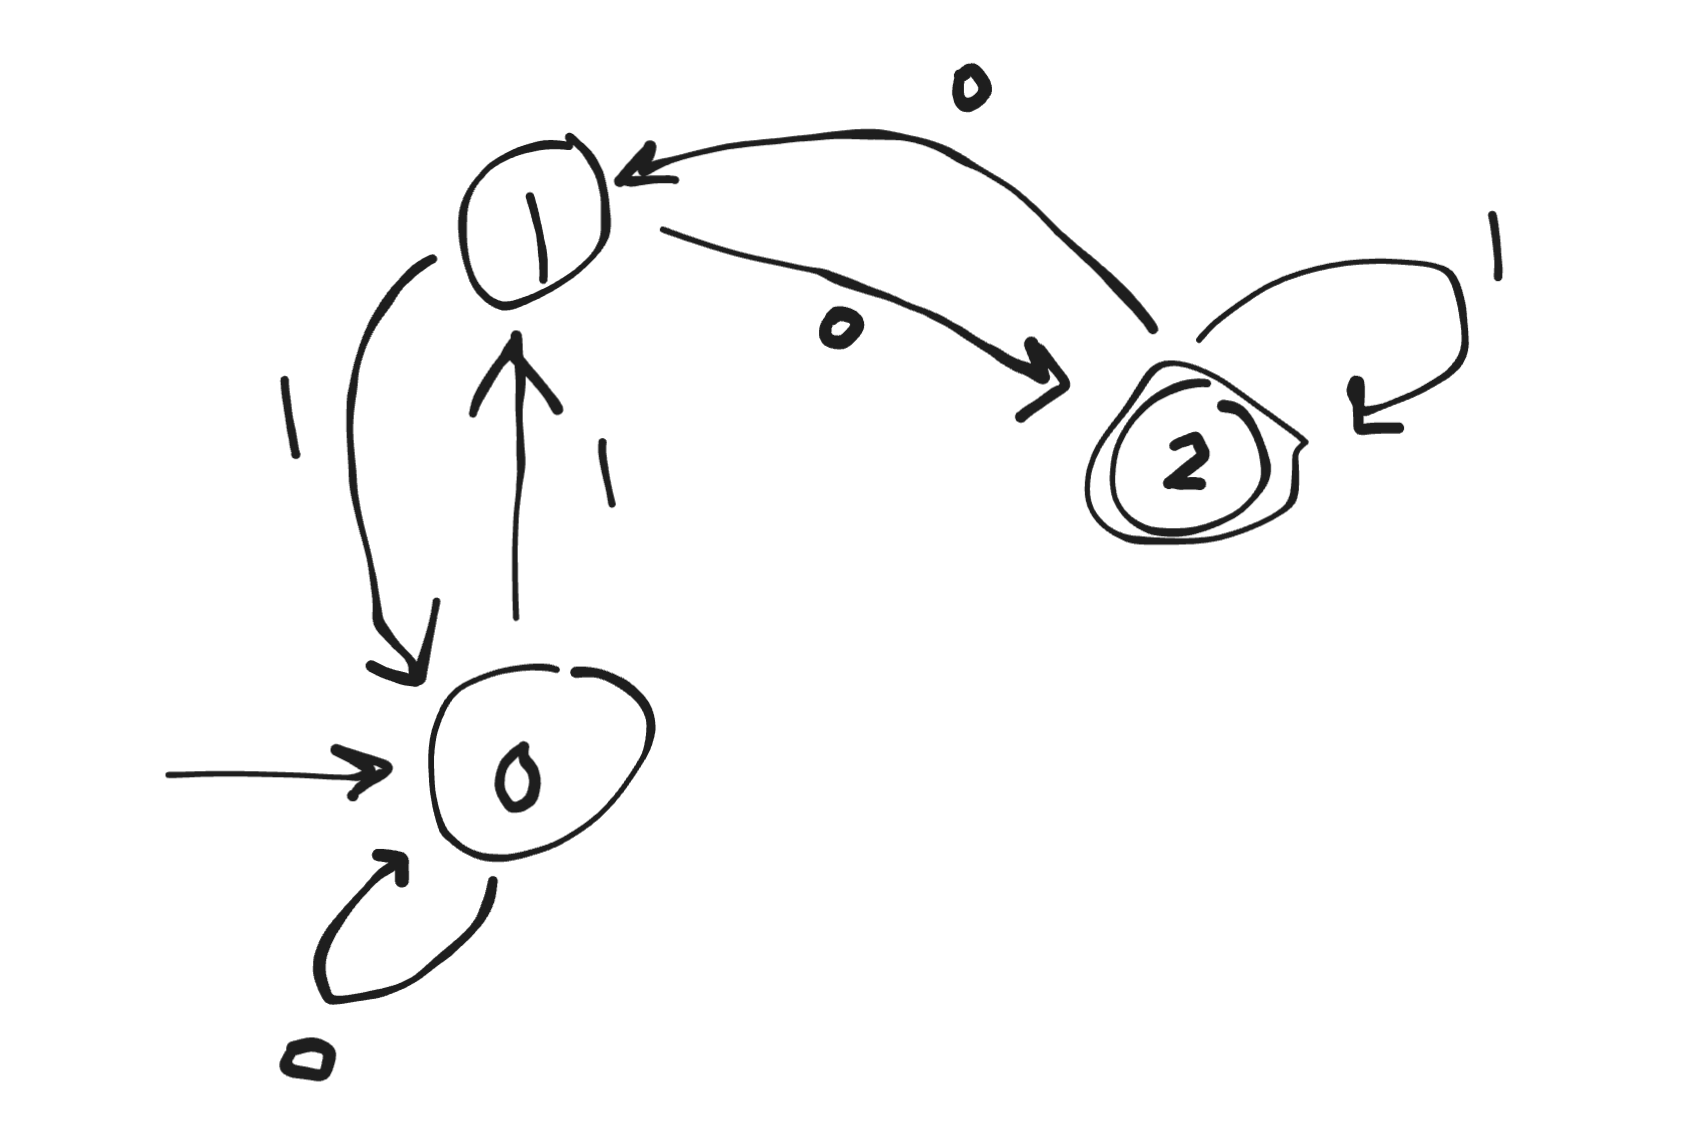
\includegraphics[width=0.7\textwidth]{DFA-10b.png}

\subsection*{Part (c)}
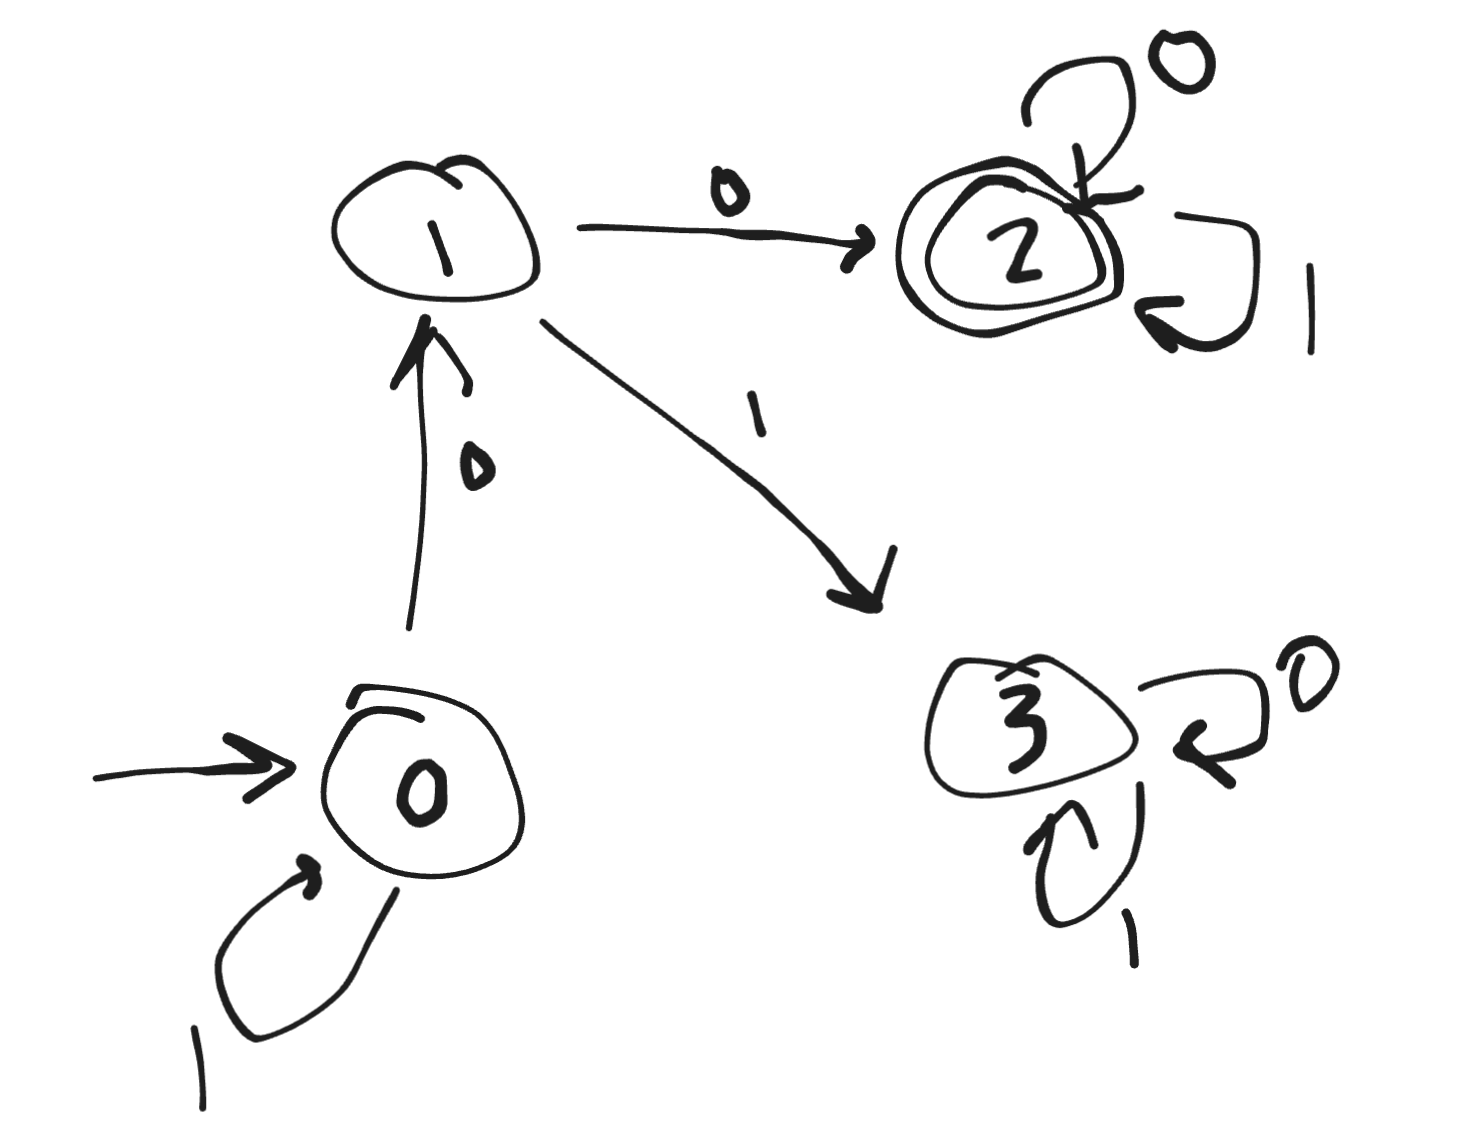
\includegraphics[width=0.7\textwidth]{DFA-10c.png}
\section*{Problem 11}
\subsection*{Part (a)}
Figure 1 from the book accepts binary numbers $n$ with an odd number of $1$s and rejects otherwise, so the Thue-Morse sequence is $2$-automatic.

\subsection*{Part (b)}
Given the diagram from problem 10c along with the function $f(q_0) = f(q_1) = f(q_3) = 0$, $f(q_2) = 1$, we have that $f(\text{final state}) = 1$ iff $\varepsilon_n = 1$, so the paper-folding sequence is $2$-automatic.

\subsection*{Part (c)}
Define a DFA where both states $q_0, q_1$ are mapped to $q_0$ when the input is $1$ and states are switched when the input is $0$. Since the state is swapped whenever a factor of $2$ is introduced and resets when a $1$ is added, the DFA keeps track of the parity of the number of factors of $2$.

\subsection*{Part (d)}
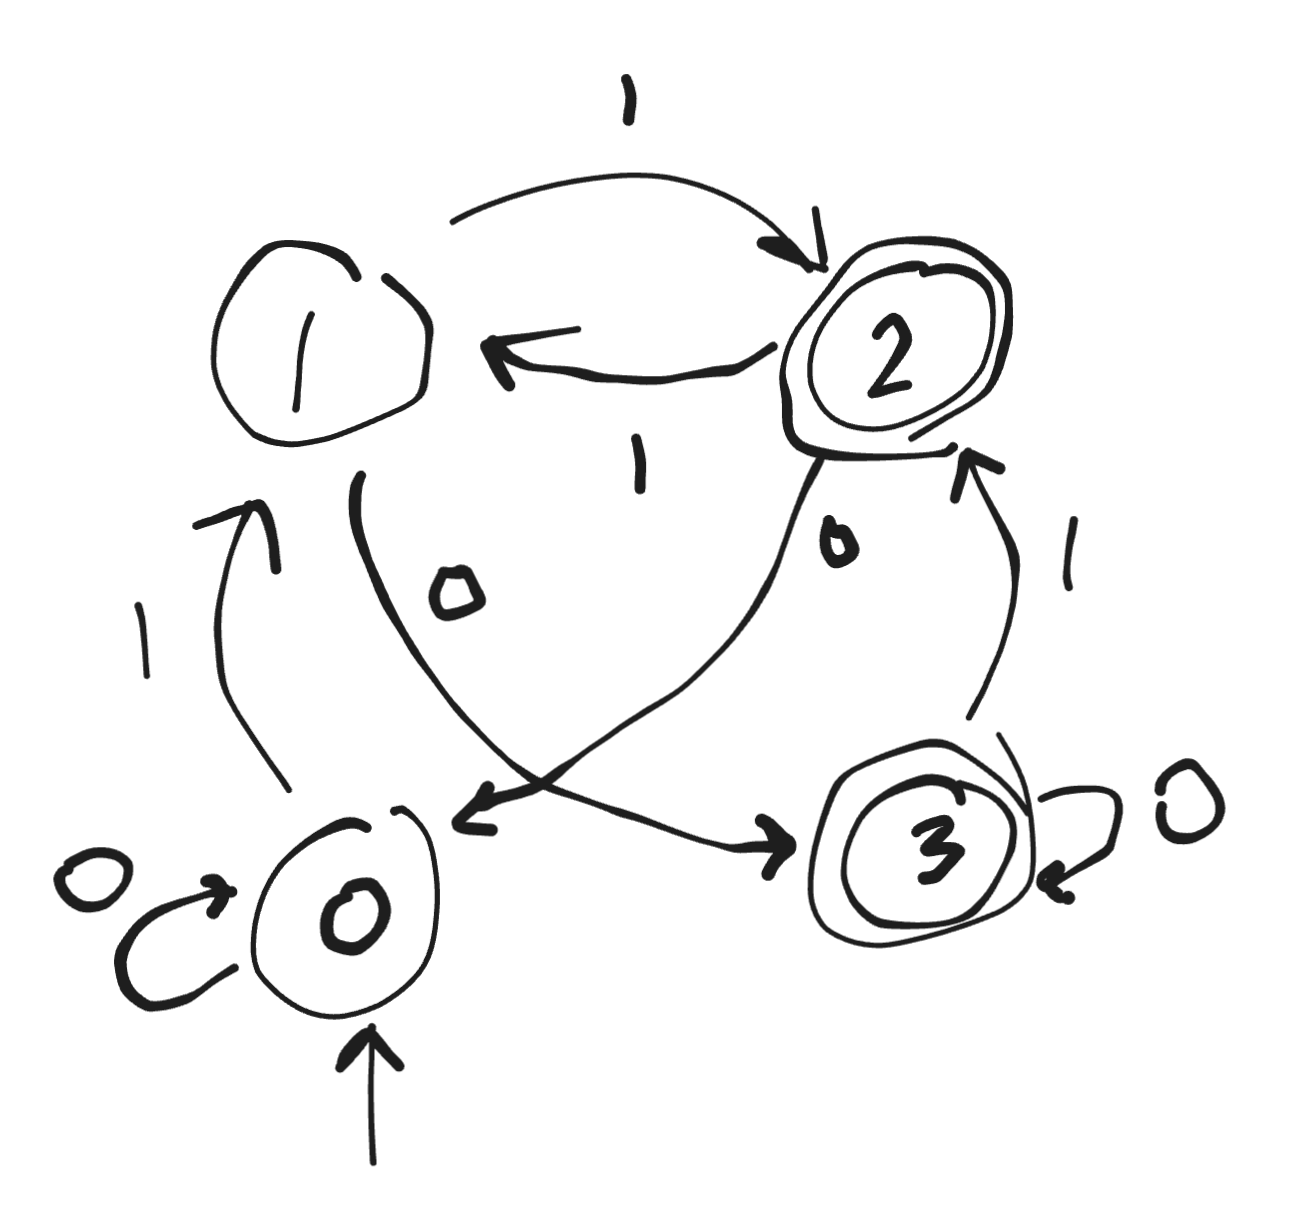
\includegraphics[width=0.7\textwidth]{DFA-11d.png}

The above DFA diagram shows a DFA that accepts $n$ iff the $n$th term in the Rudin-Shapiro sequence is $1$, so it is $2$-automatic.

\subsection*{Part (e)}
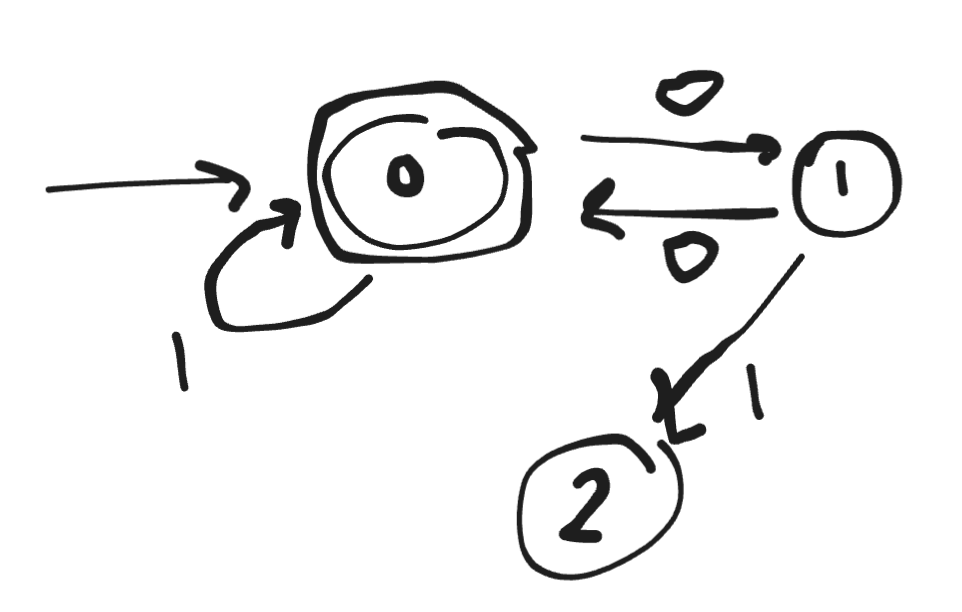
\includegraphics[width=0.7\textwidth]{DFA-11e.png}

The above DFA diagram shows a DFA that accepts $n$ iff the $n$th term in the Baum-Sweet sequence is $1$, so it is $2$-automatic.

\section*{Problem 13}
Assume a DFA reads base-$k$ digits and outputs $a_n$. Each base-$k$ digit corresponds to a word of length $m$ in base $k$, so for each symbol $d \in \{0, \ldots, k^m - 1\}$, we can write $d$ in base $k$ as an $m$-digit string and define the new transition function to simulate the DFA reading those digits in a sequence.

Now, assume a DFA reads base-$k^m$ digits. To read base-$k$, we need to group digits into blocks of size $m$. So the automaton must remember it's current state in the original machine, how many digits of the current $m$-block it has read, and the value of the block so far. Since $m$ is fixed, that only requires a finite number of states, so the result is still a DFA.

\end{document}